% !TEX root = ../Thesis.tex

\chapter{Numerical results}

This is where you show that the novel `thing' you described in Chapter~\ref{cap:proposal} is, indeed, much better than the existing versions of the same.

You will probably use figures (try to use a high-resolution version), graphs, tables, and so on. An example is shown in Figure~\ref{fig:dave}.

\begin{figure}[htbp]
\begin{center}
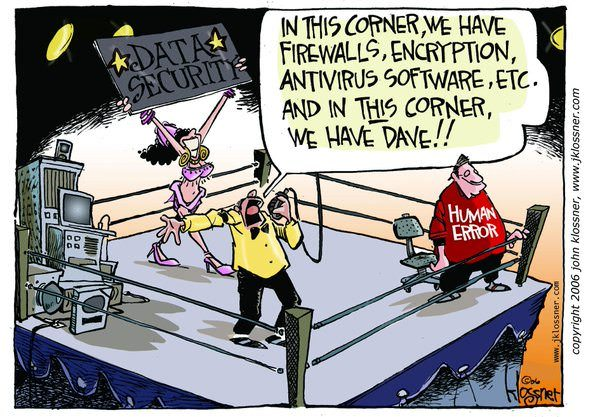
\includegraphics[width=.7\textwidth]{DaveSecurity}
\caption{Network Security - the sad truth}
\label{fig:dave}
\end{center}
\end{figure}

Note that, likewise tables and listings, you shall not worry about where the figures are placed. Moreover, you should not add the file extension (LaTeX will pick the `best' one for you) or the figure path.
